\hypertarget{a00352}{}\section{Token protocol}
\label{a00352}\index{Token protocol@{Token protocol}}
Communicating parameter state with the host. 

\hypertarget{a00352_advancedTopics_parameterUpdates_tokenProtocol_contents}{}\subsection{On this page}\label{a00352_advancedTopics_parameterUpdates_tokenProtocol_contents}
\begin{DoxyItemize}
\item \hyperlink{a00352_tokenProtocol_introductionToTokens}{An Introduction to Tokens} \item \hyperlink{a00352_tokenProtocol_standardTokenOperation}{Basic Token Operation}\end{DoxyItemize}
 \hypertarget{a00352_tokenProtocol_introductionToTokens}{}\subsection{An Introduction to Tokens}\label{a00352_tokenProtocol_introductionToTokens}
One way in which a plug-\/in can communicate with the \char`\"{}outside world\char`\"{} is through Shared Data Services, also known as the Token System. This is a mechanism that allows Pro Tools to share parameter information with external hardware and software modules. While the A\+A\+X S\+D\+K only uses the Token System indirectly, knowing how it works will provide a good understanding of how linked parameters should operate.

\hypertarget{a00352_tokenProtocol_introductionToTokens_touch}{}\subsubsection{Touch}\label{a00352_tokenProtocol_introductionToTokens_touch}
Touch tokens inform the system of user interaction with a parameter. When a parameter is being touched the system knows to stop sending automation data to the plug-\/in and just use the S\+E\+T value of the parameter. It is also used to tell the system when to start/stop recording new automation data.

In A\+A\+X, the touch message is sent to the host by \hyperlink{a00086_a30fdb67042b8dc9fb42fa9023ed9cce0}{A\+A\+X\+\_\+\+I\+Automation\+Delegate\+::\+Post\+Touch\+Request()}. The most common way to call this method is via the following methods\+:


\begin{DoxyCode}
\textcolor{keyword}{class }\hyperlink{a00099}{AAX\_IEffectParameters}
\{
    \textcolor{keyword}{virtual} \hyperlink{a00149_a4d8f69a697df7f70c3a8e9b8ee130d2f}{AAX\_Result} \hyperlink{a00061_ae82e80cbfd9cb837f8101a85f06856ba}{TouchParameter} ( \hyperlink{a00149_a1440c756fe5cb158b78193b2fc1780d1}{AAX\_CParamID} inParameterID );
    \textcolor{keyword}{virtual} \hyperlink{a00149_a4d8f69a697df7f70c3a8e9b8ee130d2f}{AAX\_Result} \hyperlink{a00061_a2caf1b7b8e2dad62cf96f144479dee60}{ReleaseParameter} ( \hyperlink{a00149_a1440c756fe5cb158b78193b2fc1780d1}{AAX\_CParamID} inParameterID 
      );
\};

\textcolor{keyword}{class }\hyperlink{a00108}{AAX\_IParameter}
\{
    \textcolor{keyword}{virtual} \textcolor{keywordtype}{void} \hyperlink{a00108_a74c71243313f9d817c8bcb77550969aa}{Touch} ();                     
    \textcolor{keyword}{virtual} \textcolor{keywordtype}{void} \hyperlink{a00108_a3d4869d9b6ec03d4f95f33f56479756f}{Release} ();
\};
\end{DoxyCode}


However, A\+A\+X plug-\/ins will rarely need to call these methods directly since the \hyperlink{a00033}{A\+A\+X\+\_\+\+C\+Parameter} and \hyperlink{a00018}{A\+A\+X\+\_\+\+C\+Effect\+Parameters} implementations will automatically handle parameter touch and release tokens whenever a new value is set on the parameter by the plug-\/in.

Other clients besides the plug-\/in may touch a parameter. Since the T\+O\+U\+C\+H token can come from a control surface the touch state will actually come back to the plug-\/in via\+:


\begin{DoxyCode}
\textcolor{keyword}{class }\hyperlink{a00099}{AAX\_IEffectParameters}
\{
    \textcolor{keyword}{virtual} \hyperlink{a00149_a4d8f69a697df7f70c3a8e9b8ee130d2f}{AAX\_Result} \hyperlink{a00061_a93483f44315bdf3adf60bf5bf773fbb8}{UpdateParameterTouch} ( 
      \hyperlink{a00149_a1440c756fe5cb158b78193b2fc1780d1}{AAX\_CParamID} iParameterID, \hyperlink{a00149_aa216506530f1d19a2965931ced2b274b}{AAX\_CBoolean} iTouchState );
\};
\end{DoxyCode}


This method is mainly important for \hyperlink{a00354}{linked parameters}.


\begin{DoxyImage}
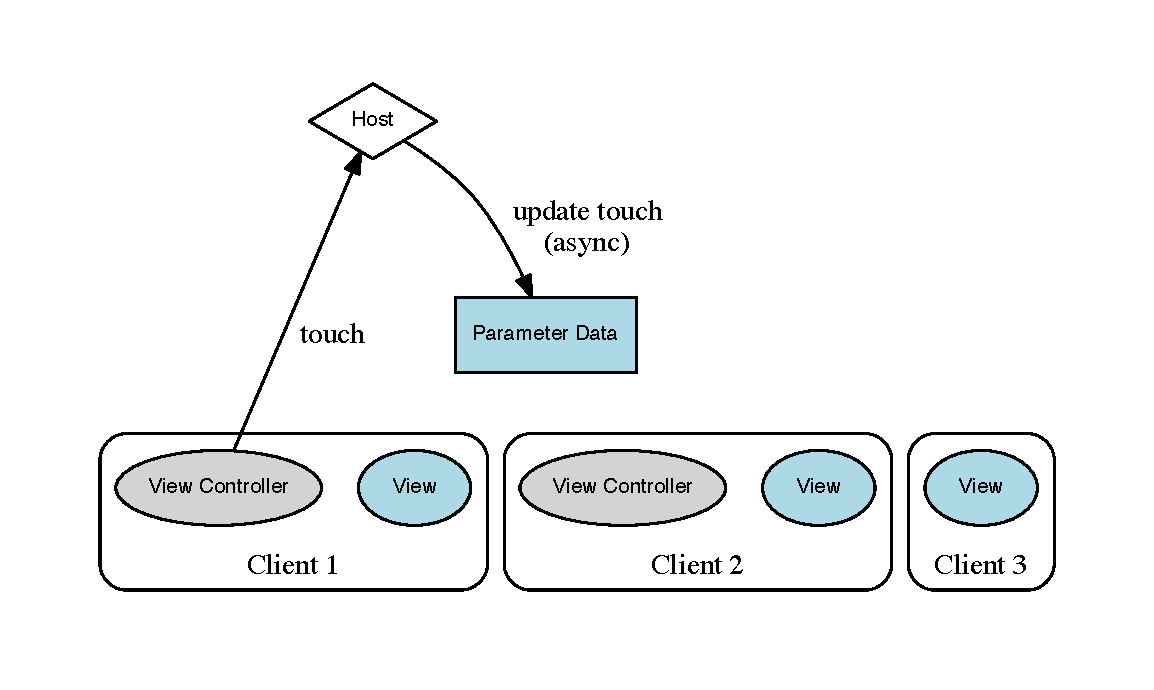
\includegraphics[width=\textwidth,height=\textheight/2,keepaspectratio=true]{dot_aax_parameter_entities_touch_handled}
\caption{Touch request from a view controller, with resulting async touch update}
\end{DoxyImage}
 \hypertarget{a00352_tokenProtocol_introductionToTokens_set}{}\subsubsection{Set}\label{a00352_tokenProtocol_introductionToTokens_set}
S\+E\+T tokens can come from many different locations\+: the plug-\/in G\+U\+I, a control surface, loading a chunk or automation playback. Eventually the value of a S\+E\+T token comes into the plug-\/in and that\textquotesingle{}s when the internal value of the parameter gets updated. In A\+A\+X the S\+E\+T token will be sent as a result of calling the following method\+:


\begin{DoxyCode}
\textcolor{keyword}{class }AAX\_CParemeter<T>
\{
    \textcolor{keywordtype}{void} SetValue ( T newValue );
\};
\end{DoxyCode}


which will be called from many other supporting methods\+:


\begin{DoxyCode}
\textcolor{keyword}{class }\hyperlink{a00033}{AAX\_CParameter}<T>
\{
    \textcolor{keywordtype}{bool} \hyperlink{a00033_a2089ea0d243087c562ce8b1bd89a495a}{SetValueWithBool} ( \textcolor{keywordtype}{bool} value );
    \textcolor{keywordtype}{bool} \hyperlink{a00033_aaf45f020a267f894429b4a75ddbe9c6c}{SetValueWithInt32} ( int32\_t value );
    \textcolor{keywordtype}{bool} \hyperlink{a00033_ab3f589671d20c826859b4398e96ee9bb}{SetValueWithFloat} ( \textcolor{keywordtype}{float} value );
    \textcolor{keywordtype}{bool} \hyperlink{a00033_a7551c4071f91cb48103b5a8dda8f73eb}{SetValueWithDouble} ( \textcolor{keywordtype}{double} value );
    \textcolor{keywordtype}{void} \hyperlink{a00033_a9ae87f0a8655c68ac7c59bec3f476c48}{SetToDefaultValue} ();
    \textcolor{keywordtype}{void} \hyperlink{a00033_ac4f8ae8c5ecb2cd04ebc3aa2523449f7}{SetNormalizedValue} ( \textcolor{keywordtype}{double} normalizedNewValue );
    \textcolor{keywordtype}{bool} \hyperlink{a00033_aa9194daefda8f6491849819fb25a73d2}{SetValueFromString} ( \textcolor{keyword}{const} \hyperlink{a00042}{AAX\_CString} & newValueString );
\};
\end{DoxyCode}


When a S\+E\+T token enters the system from the G\+U\+I, control surface or automation the value comes bak to the plug-\/in via the following method\+:


\begin{DoxyCode}
\textcolor{keyword}{class }\hyperlink{a00018}{AAX\_CEffectParameters}
\{
    \hyperlink{a00149_a4d8f69a697df7f70c3a8e9b8ee130d2f}{AAX\_Result} \hyperlink{a00018_a56a9f41a975b48f583655db7b43aae5a}{UpdateParameterNormalizedValue} ( 
      \hyperlink{a00149_a1440c756fe5cb158b78193b2fc1780d1}{AAX\_CParamID} iParameterID, \textcolor{keywordtype}{double} aValue, \hyperlink{a00206_a30be0398faf20c6b121239eb9399f3f7}{AAX\_EUpdateSource} inSource);
\};
\end{DoxyCode}


At this point the internal contents of the plug-\/in are set.


\begin{DoxyImage}
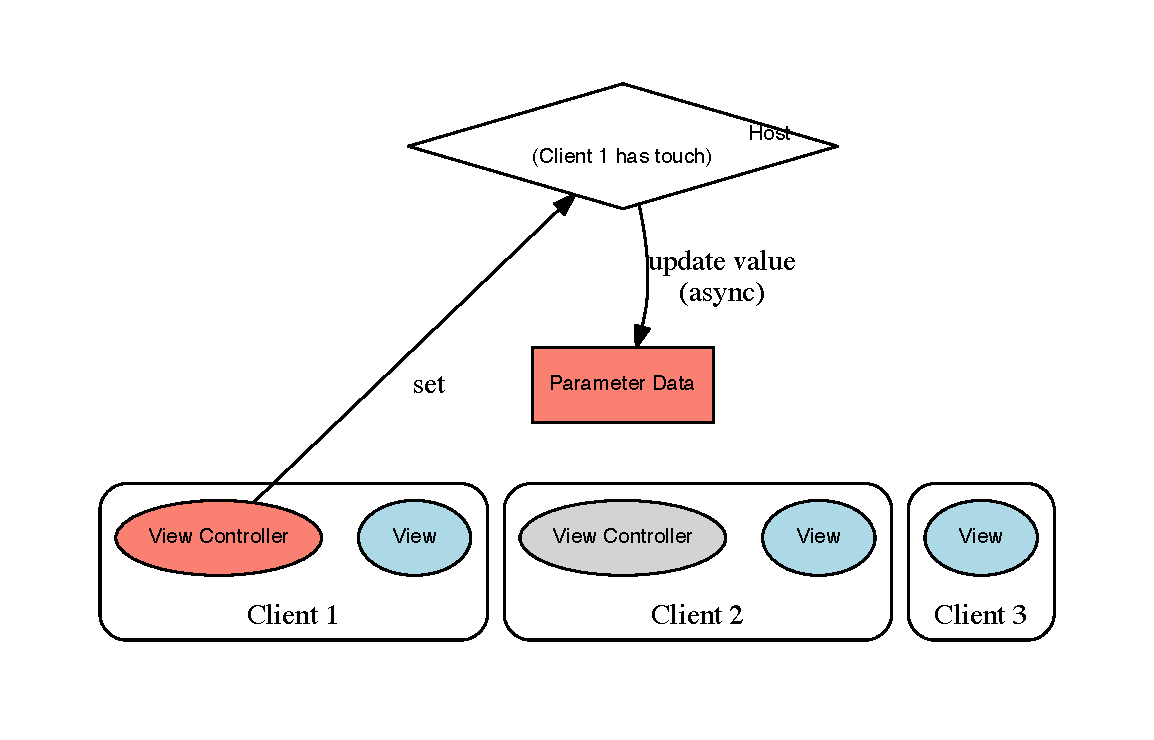
\includegraphics[width=\textwidth,height=\textheight/2,keepaspectratio=true]{dot_aax_parameter_entities_update}
\caption{Set token asynchronously changes state of the parameter data}
\end{DoxyImage}
 \hypertarget{a00352_tokenProtocol_introductionToTokens_update}{}\subsubsection{Update}\label{a00352_tokenProtocol_introductionToTokens_update}
An update token is generated when the internal value of a parameter has been set. G\+U\+Is and control surfaces listen for U\+P\+D\+A\+T\+E tokens to update the displayed values. In A\+A\+X the U\+P\+D\+A\+T\+E token is sent by calling the following method\+:


\begin{DoxyCode}
\textcolor{keyword}{class }\hyperlink{a00033}{AAX\_CParameter}<T>
\{
    \textcolor{keywordtype}{void} \hyperlink{a00033_a8a70b3c8bcff486c18e9a6e5c8ce4dda}{UpdateNormalizedValue} ( \textcolor{keywordtype}{double} newNormalizedValue );
\};
\end{DoxyCode}


All views of the parameter are then asynchronously notified that the value has changed. The plug-\/in G\+U\+I is notified via a call to \hyperlink{a00060_a45b468fef806611581f748af9301ab4d}{A\+A\+X\+\_\+\+I\+Effect\+G\+U\+I\+::\+Parameter\+Updated()}.


\begin{DoxyImage}
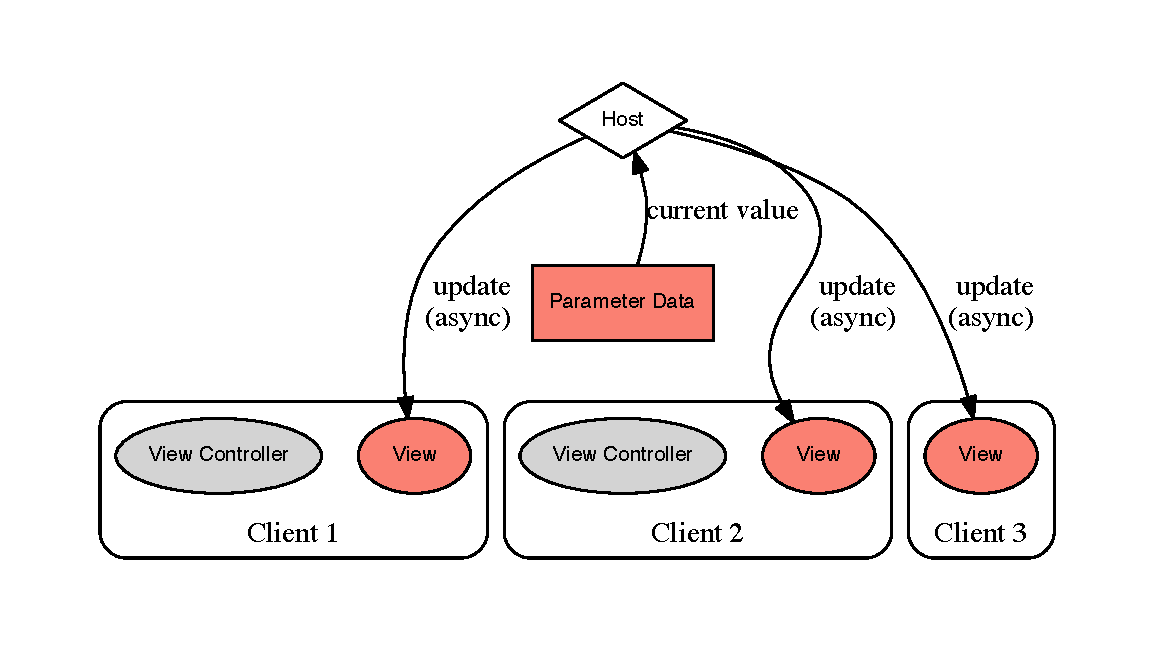
\includegraphics[width=\textwidth,height=\textheight/2,keepaspectratio=true]{dot_aax_parameter_entities_curvalue}
\caption{Update token triggers async updates to all views}
\end{DoxyImage}


 \hypertarget{a00352_tokenProtocol_standardTokenOperation}{}\subsection{Basic Token Operation}\label{a00352_tokenProtocol_standardTokenOperation}
The lists below indicate how the system works in a few different standard update scenarios. To enable logging for these events set {\ttfamily D\+T\+F\+\_\+\+A\+U\+T\+O\+M\+A\+T\+I\+O\+N=file@D\+T\+P\+\_\+\+L\+O\+W} in the \hyperlink{a00364}{Digi\+Trace} configuration file. For more detailed information about the sequence of calls used to update parameters in different situations, see \hyperlink{a00353}{Basic parameter update sequences}.

\hypertarget{a00352_tokenProtocol_standardTokenOperation_userEditing}{}\subsubsection{User Editing}\label{a00352_tokenProtocol_standardTokenOperation_userEditing}

\begin{DoxyEnumerate}
\item User clicks on a parameter in the G\+U\+I or grabs a parameter on the controls surface. A T\+O\+U\+C\+H token should be sent at this point.
\item The user changes the parameter from the G\+U\+I or controls surface. A S\+E\+T token should be sent at this point.
\item The S\+E\+T token goes into the system and comes back to the plugin via Update\+Parameter\+Normalized\+Value().
\item The plug-\/in updates it\textquotesingle{}s internal state and sends an U\+P\+D\+A\+T\+E token.
\item Repeat steps 2-\/4 while changing the parameter.
\item The user lets go of the G\+U\+I or controls surface. A T\+O\+U\+C\+H token with the released state should be sent.
\end{DoxyEnumerate}

\hypertarget{a00352_tokenProtocol_standardTokenOperation_automationPlayback}{}\subsubsection{Automation Playback}\label{a00352_tokenProtocol_standardTokenOperation_automationPlayback}

\begin{DoxyEnumerate}
\item The S\+E\+T token comes from the automation system and enters the plugin via Update\+Parameter\+Normalized\+Value().
\item The plug-\/in updates it\textquotesingle{}s internal state and sends an U\+P\+D\+A\+T\+E token.
\item Repeat steps 1-\/2 while playing back automation.
\end{DoxyEnumerate}

\hypertarget{a00352_tokenProtocol_standardTokenOperation_chunkRestoring}{}\subsubsection{Chunk Restoring}\label{a00352_tokenProtocol_standardTokenOperation_chunkRestoring}

\begin{DoxyEnumerate}
\item Plug-\/in loads the chunk.
\item The plug-\/in sets every parameters value. Another thing to note is that the
\item Set\+Value() method also contains Touch() and Release() calls. So, while setting every parameter there is a combination of T\+O\+U\+C\+H and S\+E\+T tokens sent to the system.
\item The S\+E\+T tokens comes back to the plugin via Update\+Parameter\+Normalized\+Value().
\item The plug-\/in updates it\textquotesingle{}s internal state and sends out U\+P\+D\+A\+T\+E tokens.
\end{DoxyEnumerate}

 Collaboration diagram for Token protocol\+:
\nopagebreak
\begin{figure}[H]
\begin{center}
\leavevmode
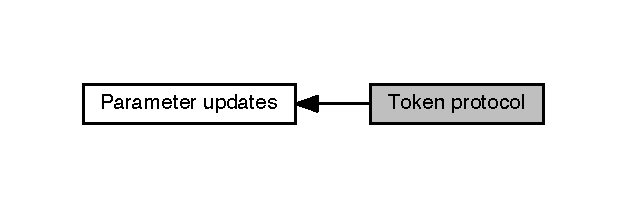
\includegraphics[width=301pt]{a00352}
\end{center}
\end{figure}
